\chapter{Frequency domain and Fourier Transform}
\noindent
Hasta ahora, hemos operado en el \textbf{dominio espacial}, donde una imagen se representa como una matriz de intensidades indexadas por coordenadas espaciales $(x, y)$. Sin embargo, Jean Baptiste Joseph Fourier demostró que cualquier función periódica puede descomponerse en una suma de senos y cosenos de diferentes frecuencias. \\

\noindent
El bloque básico de construcción es un sinusoidal:
$$A \sin(\omega x + \phi)$$
donde:
\begin{itemize}
    \item $A$ = amplitud (fuerza/intensidad)
    \item $\omega$ = frecuencia angular (qué tan rápido oscila)
    \item $\phi$ = fase (posición inicial del sinusoidal)
\end{itemize}
Agregando suficientes sinusoides a diferentes frecuencias $\omega$ con las amplitudes $A$ y fases $\phi$ correctas, se puede obtener cualquier señal periódica deseada. \\ 

\noindent
En visión por computadora, pasamos al \textbf{dominio de la frecuencia} para analizar no ``dónde'' ocurren los cambios de brillo, sino con qué \textbf{rapidez o tasa de variación} se producen en la imagen.


\section{Fourier Transform}
\begin{definicion}[Continuous Fourier Transform]
    La \tbf{Transformada de Fourier} descompone una señal continua $f(x)$ en su contenido de frecuencia al calcular, para cada frecuencia $s$, cuánto de esa frecuencia está presente:
    $$F(s) = \int_{-\infty}^{+\infty} f(x) e^{-i2\pi sx} dx$$
    Usando la fórmula de Euler $e^{i\theta} = \cos \theta + i \sin \theta$, esto esencialmente proyectar $f(x)$ sobre sinusoides de cada frecuencia $s$.
\end{definicion}

\noindent
Cada $F(s)$ es un número complejo en cada frecuencia $s$. Codifica tanto:
\begin{itemize}
    \item Amplitud (magnitud): $|F(s)| = \sqrt{\text{Re}(F)^2 + \text{Im}(F)^2}$, que indica qué tan fuerte es cada frecuencia.
    \item Fase: $\angle F(s) = \arctan \left( \frac{\text{Im}(F)}{\text{Re}(F)} \right)$, que indica el desplazamiento temporal de cada sinusoidal.
\end{itemize}

\begin{observacion}
    Definimos la Transformada de Fourier Continua para establecer la base teórica perfecta del análisis de señales. Nos proporciona el marco ideal para modelar filtros teóricos y entender cómo la luz interactúa físicamente con los sistemas ópticos de las cámaras.
\end{observacion}

\begin{definicion}[Inverse Fourier Transform]
    La \tbf{Transformada Inversa de Fourier} permite regresar al dominio espacial:
    $$f(x) = \int_{-\infty}^{+\infty} F(s) e^{i2\pi sx} ds$$
    La transformada de Fourier es invertible: $f(x) \xleftrightarrow{\mathcal{F}} F(s)$, lo que significa que no se pierde información al pasar al dominio de la frecuencia. \\
\end{definicion}


\noindent
La \textbf{Transformada de Fourier Discreta (DFT)} es la herramienta matemática que mapea una imagen desde el dominio espacial al dominio de la frecuencia.

\begin{definicion}
    Dada una imagen digital $f(x,y)$ de tamaño $M \times N$, su \tbf{discreat Fourier transform} bidimensional, denotada como $F(u,v)$, se define formalmente como:
    $$F(u,v) = \sum_{x=0}^{M-1} \sum_{y=0}^{N-1} f(x,y) e^{-j2\pi \left( \dfrac{ux}{M} + \dfrac{vy}{N} \right)}$$
    donde:
    \begin{itemize}
        \item $x, y$ son las coordenadas en el espacio.
        \item $u, v$ son las variables de frecuencia espacial.
        \item $j = \sqrt{-1}$ representa la unidad imaginaria.
    \end{itemize}
\end{definicion}

\begin{observacion}
    La DFT es la herramienta que permite aplicar toda la magia teórica de Fourier dentro de un chip o un procesador. Sin la DFT (y su implementación algorítmica ultrarrápida, la FFT o Transformada Rápida de Fourier), sería imposible que un software procesara imágenes digitalmente en tiempo real.
\end{observacion}

\begin{definicion}
    Para regresar al dominio espacial sin perder información (operación reversible), aplicamos la \textbf{Transformada Inversa Discreta de Fourier (IDFT)}:
    $$f(x,y) = \frac{1}{MN} \sum_{u=0}^{M-1} \sum_{v=0}^{N-1} F(u,v) e^{j2\pi \left( \dfrac{ux}{M} + \dfrac{vy}{N} \right)}$$
\end{definicion}

\noindent
Dado que $F(u,v)$ es un número complejo, comúnmente lo visualizamos a través de dos componentes:
\begin{enumerate}
    \item \textbf{Espectro de Magnitud ($|F(u,v)|$):} Representa la cantidad (energía) de cada frecuencia presente en la imagen. 
    $$\text{Magnitud} = |F(u,v)| = \sqrt{\text{Real}(F)^2 + \text{Imaginario}(F)^2}$$
    \item \textbf{Ángulo de Fase ($\phi(u,v)$):} Contiene la información sobre las posiciones de las ondas.
    $$\phi(u,v) = \tan^{-1} \left( \frac{\text{Imaginario}(F)}{\text{Real}(F)} \right)$$
\end{enumerate}

\section{Significado Físico de las Frecuencias en una Imagen}
Cuando pensamos en frecuencias en la vida cotidiana, pensamos en el tiempo (por ejemplo, el sonido: una onda que vibra muchas veces por segundo es un sonido agudo). Pero en las imágenes no tenemos tiempo, tenemos espacio (píxeles distribuidos en un plano $X$ e $Y$). Por lo tanto, hablamos de frecuencias espaciales.  \\

\noindent
\tbf{Regla de oro}: la frecuencia espacial mide con qué rapidez cambia el brillo (la intensidad del color) a medida que nos desplazamos caminando de un píxel al siguiente en una dirección de la imagen. \\

\noindent
¿Qué significa realmente que una imagen tenga altas o bajas frecuencias?

\subsection{Bajas Frecuencias (Low Frequencies)}
\begin{itemize}
    \item Corresponden a variaciones de intensidad muy lentas y suaves a lo largo del espacio.
    \item \textbf{¿Qué representan?} La iluminación general de la escena, los fondos homogéneos, las transiciones suaves de sombras y las formas macroscópicas estables.
    \item \tbf{Ejemplo}: imagina que caminas horizontalmente a lo largo de una foto que muestra un cielo despejado durante el atardecer. Empiezas en un azul profundo y, tras caminar 500 píxeles, el tono ha cambiado suavemente a un color naranja. El brillo ha cambiado, sí, pero le ha tomado mucho espacio hacerlo. Eso es una baja frecuencia.
\end{itemize}

\subsection{Altas Frecuencias (High Frequencies)}
\begin{itemize}
    \item Corresponden a cambios abruptos y rápidos de intensidad entre píxeles adyacentes.
    \item \textbf{¿Qué representan?} Los \textbf{bordes}, las texturas finas, los contornos nítidos de los objetos y, muy importantemente, el \textbf{ruido de alta frecuencia} (como el ruido gaussiano o de grano).
    \item \tbf{Ejemplo}: imagina que ahora caminas por una foto de una cebra. Estás sobre un píxel negro como el carbón e, inmediatamente en el píxel de al lado (a un solo píxel de distancia), la intensidad salta a un blanco deslumbrante. El cambio ha sido instantáneo y radical. Eso es una alta frecuencia.

\end{itemize}

\subsection{Información que proporciona la Transformada de Fourier}
\noindent
Al inspeccionar el espectro de magnitud centrado de una imagen, podemos extraer tres propiedades estructurales fundamentales:
\begin{enumerate}
    \item \textbf{Frequency content:} nos dice si la imagen es predominantemente suave (poca energía fuera del centro) o muy detallada/ruidosa (energía dispersa hacia los bordes del espectro).
    \item \textbf{Orientation information:} los patrones o líneas en el dominio espacial aparecen como ráfagas de energía perpendiculares en el dominio de la frecuencia, donde
    \begin{itemize}
        \item Si una imagen tiene líneas verticales fuertes (como los barrotes de una celda), la intensidad de la imagen cambia bruscamente cuando te mueves de izquierda a derecha (en el eje horizontal). Por lo tanto, en el espectro de Fourier verás una ráfaga de luz brillante alineada de forma horizontal saliendo del centro.
        \item Si la imagen tiene un horizonte marino muy marcado (horizontal), el cambio brusco ocurre al movernos de arriba a abajo. En el espectro verás una línea brillante vertical.
    \end{itemize}
    Podemos ver en la Figura \ref{fig:hpf} (que usa un filtro de paso-alto), un ejemplo de cómo la orientación de las líneas en el dominio espacial se refleja en la orientación de las ráfagas de energía en el dominio de la frecuencia.
    
    \item \textbf{Shape information:} las geometrías repetitivas o estructuras periódicas generan picos o patrones simétricos específicos en la distribución espacial de frecuencias.
\end{enumerate}

\observacion{
    Una cosa muy importante que nos da la transformada de Fourier al aplicarla a la imagen original es que se guarda la siguiente información:
    \begin{itemize}
        \item En el \tbf{centro del espectro} están almacenadas las bajas frecuencias. Las bajas frecuencias representan las formas gigantes, los fondos lisos y los cambios de luz muy lentos (por ejemplo, el color uniforme de una pared o el degradado suave del cielo).
        \item En la \tbf{periferia} (los bordes de la matriz) están almacenadas las altas frecuencias. Las altas frecuencias representan los cambios bruscos, instantáneos y afilados de color de la imagen (es decir: los bordes de los objetos, los detalles pequeños, las texturas rugosas y el ruido).
    \end{itemize}
}


\section{Filtrado Digital en el Dominio de la Frecuencia}
Una de las mayores ventajas de la DFT proviene del \textbf{Teorema de Convolución}, el cual establece que la convolución en el dominio espacial equivale a una multiplicación punto a punto en el dominio de la frecuencia:
$$f(x,y) * g(x,y) \iff F(u,v) \cdot G(u,v)$$
Esto abarata enormemente el costo computacional de aplicar filtros grandes. \\

\noindent
Tenemos estas dos igualdades también:
\begin{itemize}
    \item \tbf{Convolución en el espacio} $\leftrightarrow$ \tbf{Multiplicación en la frecuencia}
    $$\mathcal{F}[g * h] = \mathcal{F}[g] \cdot \mathcal{F}[h]$$
    \item \tbf{Multiplicación en la frecuencia} $\leftrightarrow$ \tbf{Convolución en el espacio}
    $$\mathcal{F}^{-1}[g \cdot h] = \mathcal{F}^{-1}[g] * \mathcal{F}^{-1}[h]$$
\end{itemize}

\subsection{Flujo de Trabajo Básico (Basic Workflow)}
\noindent
El proceso estándar para filtrar cualquier imagen en frecuencias consta de 4 pasos estrictos:
\begin{align*}
    \boxed{\text{Imagen } f(x,y)} &\longrightarrow \text{1. Calcular DFT} \longrightarrow \boxed{F(u,v)} \longrightarrow \text{2. Multiplicar por Máscara } H(u,v) \longrightarrow \\
    &\longrightarrow \boxed{G(u,v)} \longrightarrow \text{3. Calcular IDFT} \longrightarrow \boxed{\text{Imagen Filtrada } g(x,y)}
\end{align*}
donde cada caja representa una matriz de números complejos (en el caso de $F(u,v)$ y $G(u,v)$) o una matriz de intensidades reales (en el caso de $f(x,y)$ y $g(x,y)$), que representan la imagen en el dominio espacial o de la frecuencia respectivamente. \\

\noindent 
Tenemos los siguientes detalles del flujo:
\begin{itemize}
    \item $f(x,y)$: la imagen original que deseas filtrar, representada como una matriz de intensidades indexada por coordenadas espaciales.
    \item $F(u,v)$: obtienes una nueva matriz del mismo tamaño, pero cuyos valores ahora son números complejos que representan frecuencias espaciales ($u$ para la frecuencia horizontal y $v$ para la vertical). Las bajas frecuencias se concentran típicamente en el centro y las altas en la periferia.
    \item $H(u,v)$: es la matriz filtro llamada Máscara o Función de Transferencia. Esta máscara actúa como un "atenuador" o un ecualizador.
    \item $G(u,v)$: obtienes un nuevo espectro modificado, donde las frecuencias que querías eliminar se han convertido en $0$ y las que querías conservar se han quedado intactas.    
    \item $g(x,y)$: obtienes la imagen filtrada de vuelta en el dominio espacial. Si usaste un pasa-bajas, verás la imagen suavizada; si usaste un pasa-altas, verás solo sus bordes marcados.
\end{itemize}
\noindent
Matemáticamente, el proceso de filtrado se expresa como:
$$g(x,y) = \mathcal{F}^{-1} \{ F(u,v) \cdot H(u,v) \}$$
donde $H(u,v)$ es la \tbf{función de transferencia del filtro} (filtro atenuador o máscara).


\section{Tipos de Filtros}
\noindent
En esta sección, nos centraremos en dos tipos de filtros fundamentales: el \textbf{filtro pasa-bajas} y el \textbf{filtro pasa-altas}. Ambos son herramientas esenciales para la mejora de imágenes (\tbf{image enhancement}), cada uno con aplicaciones específicas en la reducción de ruido y el realce de detalles respectivamente. \\

\noindent
Podemos ver un ejemplo de ambos filtros aplicados a la misma imagen en la Figura \ref{fig:hpf-lpf}.

\begin{figure}
    \centering
    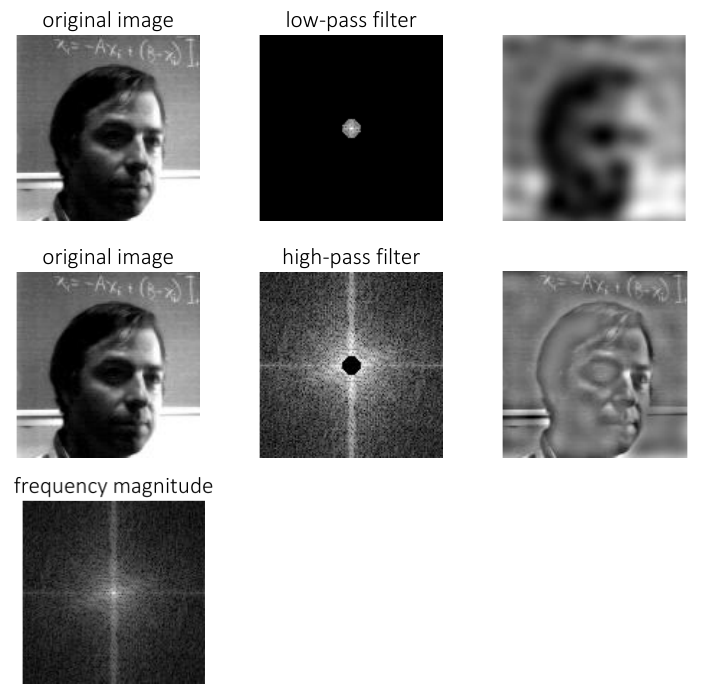
\includegraphics[width=0.8\textwidth]{img/hpf-lpf.png}
    \caption{Ejemplo de frequency magnitude, and LPF and HPF aplicados a la misma imagen.}
    \label{fig:hpf-lpf}
\end{figure}

\subsection{Low-pass Filter (LPF)}
\noindent
Un filtro pasa-bajas permite el paso de las frecuencias cercanas al centro (bajas) y atenúa o elimina las frecuencias lejanas (altas), de manera que la máscara del paso-bajas es una matriz que tiene un \tbf{círculo blanco en el centro y negro en la periferia}.
\begin{itemize}
    \item \textbf{Efecto en la imagen:} elimina los cambios bruscos de intensidad.
    \item \textbf{Resultado práctico:} produce un \textbf{suavizado o desenfoque (Blur/Smoothing)} y es sumamente útil para \tbf{eliminar el ruido} de alta frecuencia.
    \item \textbf{Tipos comunes:} filtro pasa-bajas ideal (recorte abrupto que genera artefactos de \textit{ringing}), Butterworth y Gaussiano (suave y sin oscilaciones parásitas).
\end{itemize}
A low-pass filter would be a perfect rectangle in the frequency domain, such as
\begin{equation*}
    H_{ideal}(u,v) = \begin{cases}
        1 & \text{if } |s| \leq s_c \\
        0 & \text{if } |s| > s_c
    \end{cases}
\end{equation*}
Podemos ver un ejemplo en la Figura \ref{fig:lpf}.

\begin{figure}
    \centering
    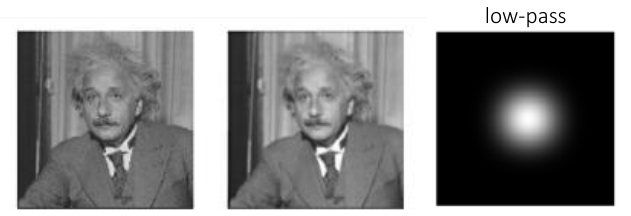
\includegraphics[width=0.8\textwidth]{img/lpf.png}
    \caption{Ejemplo filtro de paso bajo (LPF)}
    \label{fig:lpf}
\end{figure}

\subsection{High-pass Filter (HPF)}
\noindent
Un filtro pasa-altas bloquea las frecuencias bajas centrales y permite el paso de las frecuencias altas periféricas, de manera que la máscara del paso-alto es una matriz que tiene un \tbf{círculo negro (ceros) en el centro exacto y todo lo demás a su alrededor hasta las esquinas es completamente blanco (unos)}.
\begin{itemize}
    \item \textbf{Efecto en la imagen:} conserva únicamente los lugares donde la intensidad cambia rápidamente y elimina las áreas de iluminación uniforme.
    \item \textbf{Resultado práctico:} \underline{realza los bordes y detalles finos}, utilizándose de forma masiva para el afilado de imágenes (\tbf{Sharpening}) y realce de contornos.
    \item \textbf{Matriz de relación:} un filtro pasa-altas puede entenderse conceptualmente como restar la versión suavizada a la imagen original
    $$H_{\text{high}}(u,v) = 1 - H_{\text{low}}(u,v)$$
\end{itemize}
Podemos ver un ejemplo en la Figura \ref{fig:hpf}.

\begin{figure}
    \centering
    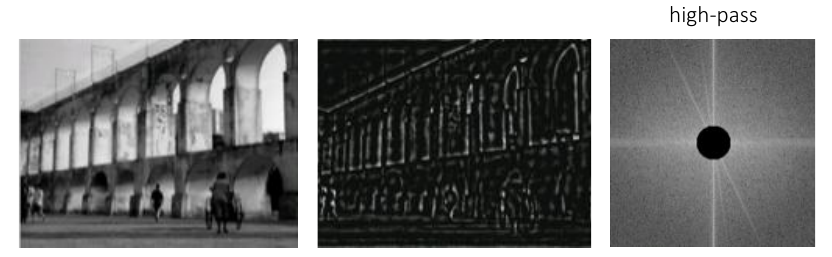
\includegraphics[width=0.8\textwidth]{img/hpf.png}
    \caption{Ejemplo filtro de paso alto (HPF)}
    \label{fig:hpf}
\end{figure}

\section{Nyquist-Shannon sampling theorem}
\begin{definicion}
    El \tbf{aliasing} es un artefacto, distorsión o error de reconstrucción que ocurre cuando una señal continua (como la luz del mundo real o los detalles finos de una escena) es digitalizada (muestreada) de forma insuficiente.  Cuando esto ocurre, las altas frecuencias (los detalles muy rápidos, pequeños o bordes afilados) pierden su identidad real y se camuflan adoptando una identidad falsa (un ``alias'') en forma de una frecuencia más baja que no existía originalmente en la escena real.  \\
\end{definicion}
\noindent
Este teorema dice que una señal continua $f(x)$ cuya transformada de Fourier $F(s)$ es cero para $|s| > s_{\text{max}}$ (es decir, es limitada en banda) puede ser perfectamente reconstruida a partir de sus muestras tomadas a una tasa:
$$f_s \geq 2 s_{\text{max}}$$
cuando $f_s < 2 s_{\text{max}}$, los componentes de alta frecuencia se pliegan (alias) sobre frecuencias más bajas, corrompiendo la reconstrucción de manera irreversible. \\

\begin{notacion}
    Conceptualmente, en una cámara fotográfica, $f_s$ es la densidad física de los píxeles en el sensor de silicio:
    \begin{itemize}
        \item Representa cuántos sensores fotosensibles individuales (fotodiodos) hay colocados por cada milímetro o pulgada cuadrada de sensor.
        \item A mayor $f_s$: Los píxeles están más juntos y apretados, lo que significa que tomas muestras de la luz de la escena real con mucha frecuencia espacial (puedes capturar detalles más pequeños).
        \item A menor $f_s$: Los píxeles están más separados entre sí, por lo que tomas muestras de la realidad de forma más espaciada y perezosa, reduciendo tu resolución espacial.
    \end{itemize}
\end{notacion}

\begin{observacion}
    Cuando hablamos de limitada en banda, significa que la señal no contiene frecuencias por encima de un cierto umbral $s_{\text{max}}$. En el contexto de las imágenes, esto se traduce en que no hay detalles más finos que un cierto nivel de detalle. Si intentamos muestrear una imagen con detalles más finos que el límite impuesto por la tasa de muestreo, esos detalles se distorsionarán y aparecerán como patrones falsos o artefactos en la imagen digitalizada. \\
\end{observacion}

\noindent
\underline{Explicación física}: Para poder registrar fielmente una oscilación periódica (un ciclo de línea blanca y línea negra), tu sensor necesita, como mínimo absoluto, colocar dos píxeles por cada ciclo: un píxel encargado de capturar la muestra del punto máximo (el blanco) y otro píxel encargado de capturar el punto mínimo (el negro). Si colocas menos de dos píxeles por ciclo, la matemática del sumatorio de la transformada discreta de Fourier ($\text{DFT}$) pierde la capacidad de distinguir esa frecuencia analógica y colapsa. \\

\noindent
La conexión con la pirámide gaussiana es la siguiente:
\begin{itemize}
    \item Cuando realizas un submuestreo de reducción a la mitad ($2\times$ downsampling), tu frecuencia de muestreo $f_s$ se reduce automáticamente a la mitad. Por lo tanto, tu nueva Tasa de Nyquist máxima permitida cae a la mitad. Si dejaras la imagen tal cual, el $s_{max}$ original violaría la nueva regla de Nyquist. Al aplicar el filtro Gaussiano justo antes de achicar la matriz, fuerzas matemáticamente a que el $s_{max}$ de la imagen disminuya, recortando las frecuencias periféricas para que queden por debajo del nuevo límite de velocidad de la imagen pequeña.
\end{itemize}
